\documentclass[12pt]{report}
\usepackage[a4paper,margin=2cm]{geometry}
\usepackage{libertine}
\usepackage[utf8]{inputenc}
\usepackage[T1]{fontenc}
\usepackage[portuges]{babel}
\usepackage{hyperref}
\usepackage{xspace}
\usepackage{booktabs}
\usepackage{multirow}
\usepackage{amsmath}
\usepackage{amsfonts}
\usepackage{amssymb}
\usepackage{listings}
\usepackage{xcolor}
\usepackage{fontawesome}
\usepackage{caption} \captionsetup[table]{skip=3pt}
\usepackage{setspace}
%\singlespacing
\onehalfspacing
%\doublespacing
%\setstretch{1.1}
\usepackage{indentfirst}
\usepackage[os=win]{menukeys}\renewmenumacro{\keys}[+]{shadowedroundedkeys}
\usepackage[lang={english},type={CC},modifier={by},version={4.0}]{doclicense}

\widowpenalty100000
\clubpenalty100000

\title{Laboratório de Sistemas Operacionais}
\author{Prof. André Leon S. Gradvohl, Dr.\\\href{mailto://exmaple@example.com}{gradvohl@ft.unicamp.br}}
\date{31 de Março de 2019}

\newcommand{\semaspas}[1]{\enquote{\texttt{#1}} {\scriptsize (sem aspas)}}

\newcommand{\Comando}[1]{{\color{blue}\texttt{#1}}}
%
\newcommand{\ComandoParametros}[2]{%
\mbox{\textcolor{blue}{\texttt{#1}}%
\xspace\textcolor{red}{\texttt{#2}}}%
}%fim ComandoParametros

\newcommand{\ComandoDoisParametros}[3]{%
\textcolor{blue}{\texttt{\textbackslash{#1}}}%
\textcolor{red}{\texttt{\{}}%
\texttt{#2}%
\textcolor{red}{\texttt{\}}}%
\textcolor{red}{\texttt{\{}}%
\texttt{#3}%
\textcolor{red}{\texttt{\}}}%
}%fim ComandoDoisParametros

\definecolor{codegreen}{rgb}{0,0.6,0}
\definecolor{codegray}{rgb}{0.5,0.5,0.5}
\definecolor{codepurple}{rgb}{0.58,0,0.82}
\definecolor{backcolour}{rgb}{0.95,0.95,0.92}

% Adiciona o : após o número da linha
\renewcommand*\thelstnumber{\the\value{lstnumber}:}
\lstdefinestyle{MyCStyle}{language=C,
  belowcaptionskip=1\baselineskip,
  breaklines=true,
  postbreak=\mbox{\textcolor{blue}{$\hookrightarrow$}\space},
  xleftmargin=\parindent,
  showstringspaces=false,
  basicstyle=\linespread{.8}\footnotesize\fontencoding{T1}\fontfamily{fvm}\selectfont,
   %identifierstyle=\color{blue},
  commentstyle=\color{codegreen},
  keywordstyle=\color{magenta},
  numbers=left,
  numberstyle=\scriptsize\color{codegray},
  stringstyle=\color{codepurple},
  frame = single, 
}

%\newcommand{\lstprompt}{\$}
%\renewcommand*\thelstnumber{\lstprompt}
\lstdefinestyle{MyBashStyle}{language=bash,
  basicstyle=\fontencoding{T1}\fontfamily{fvm}\selectfont,
  %xleftmargin=\parindent,
  xleftmargin=2.7ex,
  morecomment=[s][\color{red}]{-}{\ }, 
  morecomment=[s][\color{red}]{--}{\ },
  morekeywords={uname,gcc,git,top,grep,man,ls},%
  showstringspaces=false,
  commentstyle=\color{orange},
  keywordstyle=\color{blue},
  numberstyle=\color{codegreen}\fontencoding{T1}\fontfamily{fvm}\selectfont\,
}

\lstdefinestyle{outputStyle}{
    basicstyle=\footnotesize\fontencoding{T1}\fontfamily{fvm}\selectfont,
    identifierstyle=\color{black},
    breakatwhitespace=false,         
    breaklines=true,                 
    captionpos=b,                    
    keepspaces=true,                 
    showspaces=false,                
    showstringspaces=false,
    showtabs=false,                  
    xleftmargin=2ex,
    postbreak=\mbox{\textcolor{blue}{$\hookrightarrow$}\space},
}



\begin{document}

\maketitle
\tableofcontents
\chapter{Introdução}
O objetivo deste texto é descrever os exercícios usados no laboratório da disciplina Sistemas Operacionais. Essa disciplina é oferecida na Faculdade de Tecnologia da Universidade Estadual de Campinas (FT/UNICAMP) para os cursos Bacharelado em Sistemas de Informação e Tecnologia em Análise e Desenvolvimento de Sistemas.

Esse material pode ser utilizado por qualquer pessoa, de qualquer curso ou instituição, desde que respeitadas as condições da licença CC-BY-4.0, descrita na página \pageref{chp:licenca}. Informações de como obter o material também estão nessa página.

Supõe-se que o sistema operacional utilizado será o Linux. Portanto, todos os comandos descritos neste texto são para o Linux. Recomenda-se que o leitor navegue sequencialmente pelo texto. Assim, terá melhor aproveitamento do laboratório.

Alguns comandos básicos para o sistema Linux estão na Tabela~\ref{tab:comandosLinux} a seguir:

\begin{table}[!htb]
\begin{center}
    \caption{Lista de comandos comuns no Linux.}\label{tab:comandosLinux}
\begin{tabular}{@{}ll@{}}
\toprule
\textbf{Comando}       & \textbf{Significado} \\ \midrule
\Comando{ls} & Lista os arquivos locais.        \\
\ComandoParametros{cd}{dir}        & Muda para o diretório \textcolor{red}{\texttt{dir}}.       \\
\multirow{2}{*}{\ComandoParametros{gedit}{arquivo\,\&}}        & Abre o \textcolor{red}{\texttt{arquivo}} no editor de textos e \\
& libera o terminal para outros comandos.     \\
\ComandoParametros{unzip}{arq.zip} & Descompacta o arquivo \textcolor{red}{\texttt{arq.zip}}.   \\ \bottomrule
\end{tabular}
\end{center}
\end{table}

Todos os comandos que serão utilizados nesse tutorial serão executados no interpretador da linha de comandos (\textit{shell}), também chamado de terminal.

Há ainda algumas dicas de teclas para os usuários iniciantes no \textit{bash} (o interpretador de comandos padrão no Linux). Elas estão resumidas na Tabela~\ref{tab:teclasBash} a seguir.

\begin{table}[!htb]
\begin{center}
    \caption{Teclas úteis no \textit{bash}.}\label{tab:teclasBash}
\begin{tabular}{@{}cl@{}}
\toprule
\textbf{Tecla}     & \textbf{Significado} \\ \midrule
\keys{\arrowkeyup} & Repete o último comando.        \\
\keys{\arrowkeydown} & Repete o próximo comando.        \\
\keys{\ctrl + c} & Envia um sinal de término para o processo.\\
\keys{\tab} & Completa o nome do comando ou do arquivo.\\ 
\keys{\esc + d} & Apaga a próxima palavra a frente do cursor.\\
\keys{\ctrl + k} & Apaga do cursor até o final da linha.\\
\keys{\ctrl + a} ou \keys{Home} & Navega para o início da linha.\\
\keys{\ctrl + e} ou \keys{End} & Navega para o final da linha.\\
\keys{\ctrl + \arrowkeyleft} & Navega para a palavra anterior o cursor.\\
\keys{\ctrl+\arrowkeyright} & Navega para a próxima palavra a frente do cursor.\\
\bottomrule
\end{tabular}
\end{center}
\end{table}

\chapter{Interação com o Sistema Operacional}
Neste capítulo, veremos alguns comandos básicos para a interação com o sistema operacional Linux. 

\section{Interagindo com o sistema operacional}
O comando básico para obter informações sobre o sistema operacional está a seguir.
%\begin{center}  \texttt{uname -a} \end{center}

\begin{lstlisting}[style=MyBashStyle]
uname -a
\end{lstlisting}

Observe a saída desse comando:
\begin{lstlisting}[style=outputStyle]
Linux grid1.cna.unicamp.br 2.4.20-8 #1 Thu Mar 13 17:18:24 EST 2003 i686 athlon i386 GNU/Linux
\end{lstlisting}

Entre as informações presentes na saída desse comando estão:
\begin{itemize}
\setlength{\itemsep}{1pt}\setlength{\parskip}{0pt}  \setlength{\parsep}{0pt}
\item o nome do sistema operacional;
\item o nome da máquina;
\item versão do kernel;
\item plataforma de hardware.
\end{itemize}

\subsection{Exercício}
Utilize o comando \ComandoParametros{uname}{-a} em sua máquina e tente identificar a saída do comando.


\subsection{Mais informações sobre a distribuição do sistema operacional}
Outra possibilidade para obter mais informações sobre a distribuição do sistema operacional utilizado é consultar o arquivo \texttt{/etc/os-release}. Para isso use o comando a seguir.

\begin{lstlisting}[style=MyBashStyle]
cat /etc/os-release 
\end{lstlisting}

Observe a saída que o comando anterior produz.
\begin{lstlisting}[style=outputStyle]
NAME="Rocky Linux"
VERSION="9.5 (Blue Onyx)"
ID="rocky"
ID_LIKE="rhel centos fedora"
VERSION_ID="9.5"
PLATFORM_ID="platform:el9"
PRETTY_NAME="Rocky Linux 9.5 (Blue Onyx)"
ANSI_COLOR="0;32"
LOGO="fedora-logo-icon"
CPE_NAME="cpe:/o:rocky:rocky:9::baseos"
HOME_URL="https://rockylinux.org/"
VENDOR_NAME="RESF"
VENDOR_URL="https://resf.org/"
BUG_REPORT_URL="https://bugs.rockylinux.org/"
SUPPORT_END="2032-05-31"
ROCKY_SUPPORT_PRODUCT="Rocky-Linux-9"
ROCKY_SUPPORT_PRODUCT_VERSION="9.5"
REDHAT_SUPPORT_PRODUCT="Rocky Linux"
REDHAT_SUPPORT_PRODUCT_VERSION="9.5"
\end{lstlisting}

Dentre as informações apresentadas estão o nome da distrição Linux (nesse caso, \enquote{\texttt{Rocky Linux}}), a versão (\enquote{\texttt{9.5 (Blue Onyx)}}) e outros detalhes específicos da versão do sistema operacional utilizado.

\section{Obtendo informações sobre o hardware}
Para obter informações sobre o hardware no qual o sistema operacional está funcionando, utilizaremos dois comandos. 

\subsection{Informações sobre a unidade central de processamento}
Para buscar informações sobre a unidade central de processamento (CPU), utilizaremos o comando  \Comando{lscpu}. Esse comando buscará informações armazenadas no arquivo \texttt{/proc/cpuinfo} e em outros locais específicos do sistema operacional.

\subsection{Exercício}
Utilize o comando \Comando{lscpu} em sua máquina e tente identificar quais as informações esse comando fornece.

Depois, use o comando a seguir e verifique que informações esse comando fornece. Compare a saída do comando \Comando{lscpu} com a saída desse comando.

\begin{lstlisting}[style=MyBashStyle]
cat /proc/cpuinfo
\end{lstlisting}


\subsection{Informações sobre a memória}
Para obter informações sobre a memória, podemos utilizar o comando \Comando{lsmem}. Esse comando trará, resumidamente, as informações sobre a memória. 

Dentre essas informações que o comando \Comando{lsmem} provê estão a faixa de endereços de memória (\texttt{RANGE}), o tamanho de cada faixa (\texttt{SIZE}), o estado (\texttt{STATE}), se é um bloco removível, e os blocos correspondentes (\texttt{BLOCK}). Ao final, o comando indica o tamanho do bloco de memória e a quantidade total de memória \textit{online} e \textit{offline} (desativada).

Para informações mais completas sobre a memória do computador que você está utilizando, abra o arquivo \texttt{/proc/meminfo}.

\subsection{Exercício}
Utilize o comando \Comando{lsmem} em sua máquina e tente identificar quais as informações esse comando fornece.

Depois, use o comando \semaspas{\Comando{cat} \texttt{/proc/meminfo}} e verifique que informações esse comando fornece. Compare a saída do comando \Comando{lsmem} com a saída desse comando.


\section{Informações sobre o sistema por meio de um código-fonte}
Todas as informações sobre o hardware, isto é, informações sobre CPU e memória podem ser obtidas por meio de um código-fonte. Para isso, observe o código fonte a seguir.

\clearpage
\lstinputlisting[style=MyCStyle]{./Programas/InfoSistema/infoSistema.c}

\subsection{Exercício}
Para ver o resultado do programa anterior, compile-o e execute-o. Antes de compilar o programa, mude para o diretório onde se encontra o arquivo  \texttt{infoSistema.c}, com o seguinte comando:

\begin{lstlisting}[style=MyBashStyle]
cd InfoSistema
\end{lstlisting}

Fique atento, pois o interpretador da linha de comando (o \textit{shell}) diferencia as letras maiúsculas das letras minúsculas.

Para compilar o programa, utilize o comando a seguir.
\begin{lstlisting}[style=MyBashStyle]
gcc infoSistema.c -o infoSistema
\end{lstlisting}

Para executar o programa, execute a linha de comando a seguir.
\begin{lstlisting}[style=MyBashStyle]
./infoSistema
\end{lstlisting}

\section{Obtendo informações sobre processos}
Existem dois comandos para obtenção de informações sobre processos: \Comando{ps} e \Comando{top}.

O comando \Comando{ps} informa o status dos processos de forma sucinta. As informações que o comando \Comando{ps} apresenta são:

\begin{itemize}
\setlength{\itemsep}{1pt}\setlength{\parskip}{0pt}  \setlength{\parsep}{0pt}
\item \texttt{PID}: identificador do processo;
\item \texttt{TTY}: terminal onde o processo está sendo executado;
\item \texttt{TIME}: tempo de processamento;
\item \texttt{CMD}: comando instanciado.
\end{itemize}

O comando \Comando{top} é um pouco mais poderoso, pois reporta mais informações.  Entre tais informações estão:

\begin{itemize}
\setlength{\itemsep}{1pt}\setlength{\parskip}{0pt}  \setlength{\parsep}{0pt}
\item tempo em que o sistema está no ar;
\item carga média do sistema;
\item informações da CPU:
\begin{itemize}
\setlength{\itemsep}{1pt}\setlength{\parskip}{0pt}  \setlength{\parsep}{0pt}
\item porcentagem de tempo dedicada aos processos do usuário;
\item porcentagem de tempo dedicada aos processos do sistema;
\item porcentagem de tempo sem processamento (\textit{idle}).
\end{itemize}
\item informações sobre a memória:
\begin{itemize}
\setlength{\itemsep}{1pt}\setlength{\parskip}{0pt}  \setlength{\parsep}{0pt}
\item memória total;
\item memória  livre;
\item memória  compartilhada;
\end{itemize}
\item informações sobre os processos:
\begin{itemize}
\setlength{\itemsep}{1pt}\setlength{\parskip}{0pt}  \setlength{\parsep}{0pt}
\item \texttt{PID}: identificador do processo;
\item \texttt{USER}: nome do usuário;
\item \texttt{PRI}: prioridade;
\item \texttt{SIZE}: tamanho do processo em kbytes;
\item \texttt{RSS}: tamanho total de memória física do processo;
\item \texttt{SHARE}: tamanho total de memória compartilhada;
\item \texttt{STAT}:  estado do processo, que pode ser \texttt{S}  (\textit{sleeping}) ou \texttt{R} (\textit{running}).
\end{itemize}
\end{itemize}

\section{Exercício}
Utilize o comando \Comando{top} em sua máquina e tente identificar as informações providas pelo comando.

\chapter{Obtendo informações sobre os processos}
Neste capítulo, vamos verificar como obter informações sobre o próprio processo a partir dele mesmo.

\section{Obtendo informações sobre o processo, via programa}
É possível construir programas que interajam com o sistema operacional e obtenham algumas informações. Observe o código do programa a seguir:

\lstinputlisting[style=MyCStyle]{./Programas/Processos/infoProcesso.c}

\section{Exercício}
Compile o programa anterior e execute-o.

Antes de compilar o programa, mude para o diretório onde se encontra o arquivo  \texttt{infoProcesso.c}, com o seguinte comando:

\begin{lstlisting}[style=MyBashStyle]
cd Processos
\end{lstlisting}

Para compilar o programa utilize o comando a seguir:
\begin{lstlisting}[style=MyBashStyle]
gcc infoProcesso.c -o infoProcesso
\end{lstlisting}

\chapter{Tratamento de Sinais}

Sinais são usados para notificar um processo ou segmento de um evento particular. Pode-se comparar o tratamento de sinais com interrupções de hardware, que ocorrem quando um subsistema de hardware, por exemplo uma interface de entrada ou saída (E/S) de disco, gera uma interrupção para o processador quando a E/S é concluída.

Este evento, por sua vez, faz com que o processador chame um tratador de interrupções. Assim, o processamento subsequente pode ser feito no sistema operacional com base na fonte e da causa da interrupção.

Observe como isso pode ser feito no programa \texttt{sinais.c} a seguir

\lstinputlisting[style=MyCStyle]{./Programas/Sinais/sinais.c}

\section{Exercício}
 Antes de compilar o programa, mude para o diretório onde se encontra o arquivo \texttt{sinais.c}, com o seguinte comando:

\begin{lstlisting}[style=MyBashStyle]
cd ../Sinais
\end{lstlisting}

Agora para compilar o programa utilize o comando a seguir:
\begin{lstlisting}[style=MyBashStyle]
gcc sinais.c -o sinais.o 
\end{lstlisting}

Depois de compilado, será necessário abrir uma segunda janela do terminal. Na primeira janela, você executará o programa \texttt{./sinais.o}. 

Depois que o programa entrar em execução, tente pressionar as teclas \keys{\ctrl + c} para ver se o programa termina.

Para encerrar de fato o programa, na segunda janela, utilize o comando \Comando{kill} para enviar um sinal de término para o programa. Para isso, utilize o comando a seguir:

\begin{lstlisting}[style=MyBashStyle]
kill -QUIT <pid>
\end{lstlisting}

\noindent onde \texttt{<pid>} é o identificador do processo na primeira janela.

Importante: para saber o identificador do processo \texttt{./sinais} que está em execução na primeira janela, use o comando a seguir:

\begin{lstlisting}[style=MyBashStyle]
ps -ef | grep sinais.o
\end{lstlisting}


\chapter{Disparando vários processos}
A primitiva \texttt{fork()} é utilizada para, a partir de um processo, criar outro processo com as mesmas características do primeiro. Na verdade, a primitiva \texttt{fork()} faz uma cópia do processo pai em um processo filho, fazendo com que ambos continuem a sua execução do ponto imediatamente posterior à  primitiva \texttt{fork()}.

A primitiva \texttt{fork()} tem três saídas distintas:
\begin{itemize}
\setlength{\itemsep}{1pt}\setlength{\parskip}{0pt}  \setlength{\parsep}{0pt}
\item \texttt{-1} se houve problemas (nesse caso o filho não é criado);
\item \texttt{0}, para o processo filho;
\item identificador do filho, para o processo pai.
\end{itemize}

Observe o programa a seguir e tente entender o funcionamento da primitiva \texttt{fork()}.

\lstinputlisting[style=MyCStyle]{./Programas/Processos/PaiFilho.c}

\section{Exercício}
Compile o programa anterior e execute-o.

Antes de compilar o programa, mude para o diretório onde se encontra o arquivo  \texttt{PaiFilho.c}, com o seguinte comando:

\begin{lstlisting}[style=MyBashStyle]
cd../Processos
\end{lstlisting}

Para compilar o programa utilize o comando a seguir:
\begin{lstlisting}[style=MyBashStyle]
gcc PaiFilho.c -o PaiFilho
\end{lstlisting}


\section{Criando processos zumbis}
Um processo zumbi é o processo que já terminou sua execução, mas que ainda está na tabela de processos por algum motivo. Um desses motivos é que, por algum \textit{bug} no sistema operacional, a tabela de processos ainda não foi atualizada, eliminando o identificador do processo.

A princípio, um processo zumbi não é um problema sério para o sistema operacional. No entanto, a presença de zumbis pode indicar \textit{bugs} no sistema ou problemas de segurança do tipo \textit{Denial of service}.

No exemplo a seguir, vamos forçar a criação de processos zumbis.

\lstinputlisting[style=MyCStyle]{./Programas/Processos/zumbi.c}

\section{Exercício}
Antes de compilar o programa \texttt{zumbi.c}, abra uma outra janela do terminal. Você precisará executar o comando \Comando{top} na segunda janela, enquanto o programa é executado na primeira.

Compile o programa \texttt{zumbi.c} com o seguinte comando:

\begin{lstlisting}[style=MyBashStyle]
gcc zumbi.c -o zumbi.o
\end{lstlisting}

Agora, execute o programa \texttt{./zumbi.o} em uma janela e na outra execute o comando a seguir:

\begin{lstlisting}[style=MyBashStyle]
top -p <id_pai> -p <id_filho>
\end{lstlisting}

Os valores para \texttt{<id\_pai>} e \texttt{<id\_filho>} serão fornecidos pelo programa \texttt{zumbi.o}.

\section{Processos pai e filho diferentes}
A princípio, a primitiva \texttt{fork()} cria um processo filho exatamente igual ao seu processo pai. Entretanto, cada um deles fica em um espaço de memória diferente.

Contudo, há situações em que é necessário que cada processo -- pai e filho -- execute códigos diferentes. No exemplo a seguir, ilustra-se a primitiva \texttt{execvp()} para executar programas diferentes a partir de um determinado processo. 

A primitiva \texttt{execvp()} faz parte de uma família de primitivas que substitui a imagem do processo atual por uma nova. A imagem de um processo são os códigos (programa) que aquele processo executa e os respectivos dados.

A sintaxe da primitiva \texttt{execvp()} é a seguinte:

\begin{lstlisting}[style=MyCStyle, frame=none]
int execvp(const char *file, char *const argv[]);
\end{lstlisting}
 
onde: 
\begin{itemize}
    \item O valor de retorno é sempre \texttt{-1}. Mas, se isso acontecer, significa que houve um erro na execução da primitiva;
    \item \texttt{file} é nome do programa;
    \item \texttt{argv[]} é um vetor de \textit{strings} com os argumentos do programa. Importante: a primeira posição do vetor \texttt{argv} deve ter o caminho completo para o programa e última posição do vetor deve ter valor \texttt{NULL}.
 \end{itemize}
 
 O exemplo a seguir ilustra o programa que representa os processos pai e filho. 
 
 \section*{\texttt{pai.c}}
 \lstinputlisting[style=MyCStyle]{./Programas/Processos/pai.c}
 
 \section*{\texttt{filho.c}}
 \lstinputlisting[style=MyCStyle]{./Programas/Processos/filho.c}
 
 \section{Exercício}
 Compile os programas \texttt{pai.c} e \texttt{filho.c} separadamente com os seguintes comandos:

\begin{lstlisting}[style=MyBashStyle]
gcc pai.c -o pai.o
gcc filho.c -o filho.o
\end{lstlisting}


Agora execute o programa \texttt{./pai.o} e veja o resultado.

\chapter{Compartilhamento de memória}

Conforme discutido em sala de aula, é possível fazer com que dois ou mais processos compartilhem memória. Essa é uma forma para fazer com que dois processos possam se comunicar.

\section{Primitivas para compartilhamento de memória}
As primitivas usadas para fazer o compartilhamento e acesso são:
\begin{itemize}
\setlength{\itemsep}{1pt}\setlength{\parskip}{0pt}  \setlength{\parsep}{0pt}
\item \texttt{shmget}: retorna o identificador do segmento de memória compartilhado;
\item \texttt{shmat}: anexa o segmento de memória compartilhado ao espaço de endereçamento do processo;
\item \texttt{shmdt}: desanexa o segmento de memória compartilhado ao espaço de endereçamento do processo.
\end{itemize}

Observe o que os programas a seguir fazem. O primeiro é o programa \texttt{shm\_serv.c} que disponibiliza um segmento de memória. O segundo é o programa \texttt{shm\_cli.c} que acessa o segmento compartilhado.

\section*{\texttt{shm\_serv.c}}
\lstinputlisting[style=MyCStyle]{./Programas/CompartMem/shm_serv.c}

\newpage
\section*{\texttt{shm\_cli.c}}
\lstinputlisting[style=MyCStyle]{./Programas/CompartMem/shm_cli.c}

\section{Exercício}

Compile ambos os programas e, em seguida, execute em uma janela o programa  \texttt{shm\_serv} e em outra janela o programa \texttt{shm\_cli}.

Antes de compilar o programa, mude para o diretório onde se encontram os arquivos \texttt{shm\_serv.c} e \texttt{shm\_cli.c} , com o seguinte comando:
\begin{lstlisting}[style=MyBashStyle]
cd ../CompartMem
\end{lstlisting}


Para compilar o programa utilize as linhas de comando a seguir:
\begin{lstlisting}[style=MyBashStyle]
gcc shm_serv.c -o shm_serv
gcc shm_cli.c -o shm_cli
\end{lstlisting}

Agora, em uma das janela execute primeiro o programa \texttt{./shm\_serv.o} e, depois, na segunda janela execute o programa \texttt{./shm\_cli.o}. Veja o resultado.

\chapter{Programação \textit{Multithread}}
Outra forma de fazer duas ou mais tarefas ao mesmo tempo é utilizado \textit{multithreads}. Conforme já discutido em sala de aula, \textit{multithreads} são diferentes linhas de execução em um processo.

Existem algumas bibliotecas para trabalhar com \textit{multithreads}. Por exemplo, a POSIX \textit{Threads} (PThreads) -- que utilizaremos neste tutorial -- e a OpenMP, cujo paradigma é diferente da PThreads.

Neste tutorial, serão utilizadas as seguintes primitivas  da biblioteca PThreads:

\begin{itemize}
\setlength{\itemsep}{1pt}\setlength{\parskip}{0pt}  \setlength{\parsep}{0pt}
\item \texttt{pthread\_create()}: responsável pela criação de uma \textit{thread}.
\item \texttt{pthread\_exit()}: responsável por retornar um valor de uma \textit{thread}.
\item \texttt{pthread\_join()}: adiciona uma barreira para aguardar por uma segunda \textit{thread}.
\item \texttt{pthread\_self()}: obtém o identificador da \textit{thread}.
\end{itemize}

Na biblioteca PThreads em particular, os \textit{threads} são implementados como funções, com uma \enquote{assinatura} específica. Essa \enquote{assinatura} é um padrão que as funções devem adotar na sua declaração, conforme ilustra a Figura~\ref{fig:assinaturaThread} a seguir. 

\begin{figure}[!htb]
    \centering
    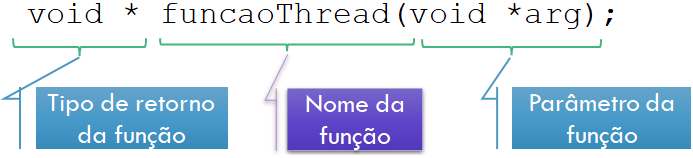
\includegraphics[width=.8\textwidth]{AssinaturaThread.png}
    \caption{Assinatura padrão de um \textit{thread}.}
    \label{fig:assinaturaThread}
\end{figure}

Note que a função que implementa um \textit{thread} deve, obrigatoriamente, retornar o tipo \enquote{\mbox{\texttt{void *}}} e receber como parâmetro um tipo \enquote{\mbox{\texttt{void *}}}. Tanto o nome da função, quanto o nome da variável passada como parâmetro pode ser definidos pelo programador.

A utilização do tipo \enquote{\mbox{\texttt{void *}}} possibilita ao programador a utilização de um endereço para qualquer tipo de dado. Contudo, para evitar que o compilador lance advertências, é preciso fazer uma conversão de tipos (\textit{cast}) para usar o conteúdo do endereço utilizado.

\section{Exemplo simples de utilização da biblioteca PThreads}
Para ilustrar a utilização da biblioteca PThreads, começaremos com um exemplo muito simples. Observe o programa \texttt{thrd.c} a seguir. O programa dispara duas \textit{threads} que \enquote{dormem} um tempo aleatório. 

Atente para os comentários que aparecem no código. Esses comentários explicam a utilização das primitivas da biblioteca PThreads.

\section*{thrd.c}
\lstinputlisting[style=MyCStyle]{./Programas/Thread/thrd.c}

A definição das funções chamadas pelo programa principal estão no arquivo a seguir.

\section*{funcoes.c}
\lstinputlisting[style=MyCStyle]{./Programas/Thread/funcoes.c}



\section{Exercício}
Compile e execute o programa anterior. Antes de compilar o programa, mude para o diretório onde se encontram os arquivos \texttt{funcoes.c} e \texttt{thrd.c} , com o seguinte comando:

\begin{lstlisting}[style=MyBashStyle]
cd ../Thread
\end{lstlisting}

Para compilar, utilize a seguinte linha de comando:

\begin{lstlisting}[style=MyBashStyle]
gcc -lpthread funcoes.c thrd.c -o thrd
\end{lstlisting}

\textcolor{orange}{\faWarning} Observação: a chave \textcolor{red}{\texttt{-lpthread}} indica que será usada a biblioteca \texttt{pthread} para Linux. Em algumas distribuições, você deve usar a chave \textcolor{red}{\texttt{-pthread}}.

\section{Passagem de parâmetros para \textit{threads}}
Vejamos agora como ocorre a passagem de parâmetros para os \textit{threads}. Antes, é preciso lembrar que na biblioteca PThreads, os \textit{threads} usam uma assinatura específica descrita na Figura~\ref{fig:assinaturaThread}. 

Para passar parâmetros para os \textit{threads}, é preciso encapsulá-los em uma estrutura e passar o endereço dessa estrutura para o \textit{thread}. Depois, já no escopo da função que implementa o \textit{thread}, esses parâmetros podem ser atribuídos às variáveis locais para serem utilizados.

\section{Retorno dos \textit{threads}}
De forma análoga à passagem de parâmetros, um \textit{thread} deve retornar um endereço de memória ou o endereço nulo (\texttt{NULL}).  

É importante destacar que, se um \textit{thread} for devolver um endereço de memória, essa posição de memória deve ter sido alocada dinamicamente. A razão para isso é que, após o término da função, todas as variáveis locais declaradas no escopo daquela função deixarão de existir. Portanto, um endereço alocado dinamicamente continuará existindo, mesmo após o término da função, até que a desalocação seja feita explicitamente (com a função \texttt{free}).

Também é preciso lembrar que esse endereço de memória devolvido ao final do \textit{thread}, precisa ser convertido para um tipo de dado específico. Caso essa operação não seja feita, o compilador poderá informar um erro de tipos na utilização da variável.

Como um exemplo de passagem de parâmetros, vejamos o exemplo a seguir. Trata-se de um programa \textit{multithread} que vai calcular a média dos números em um vetor. Nesse exemplo em particular, vamos usar um vetor de 100 posições e cada um dos quatro \textit{threads} calculará a soma parcial das suas respectivas partições (cada \textit{thread} calculará a soma de 25 elementos do vetor).

Note, logo no início da função que especifica o \textit{thread}, como os dados são extraídos do parâmetro \texttt{args} e atribuídos às variáveis locais. Essa estratégia facilita o uso posterior das variáveis na função.

Perceba também que a variável de retorno (\texttt{soma}) é um ponteiro. Esse ponteiro terá a memória alocada dinamicamente na função para que possa ser devolvida no final do \textit{thread}. 

\section*{mediaThread.c}
\lstinputlisting[style=MyCStyle]{./Programas/Thread/mediaThreads.c}

\section{Exercício}
Compile e execute o programa anterior utilizando a seguinte linha de comando:

\begin{lstlisting}[style=MyBashStyle]
gcc -lpthread auxFuncs.c mediaThreads.c -o mediaThread.o
\end{lstlisting}

\textcolor{orange}{\faWarning} Observação: a chave \textcolor{red}{\texttt{-lpthread}} indica que será usada a biblioteca \texttt{pthread} para Linux. Em algumas distribuições, você deve usar a chave \textcolor{red}{\texttt{-pthread}}.


\chapter{Problema do Produtor-Consumidor}
Um dos problemas discutidos em sala de aula é o do produtor-consumidor. Em linhas gerais, existem dois processos (ou \textit{threads}), um produtor e um consumidor, que competem pelo uso de um recurso. Nesse caso um \textit{buffer}.

O produtor gera dados e os armazena no \textit{buffer}. O consumidor, por sua vez, lê dados do buffer e os utiliza. A região crítica é o \textit{buffer}, pois apenas um dos processos deve estar utilizando o \textit{buffer} a cada instante. O sistema operacional deve prover meios de garantir essa exclusão mútua.

%Existem várias formas de se resolver esse problema. Nesse laboratório serão mostradas duas delas. A primeira utilizando \textit{multithread} e uma estratégia chamada \texttt{mutex}. A segunda usando multiprocessamento e semáforos.

\section{Problema do Produtor-Consumidor com \textit{multithreads} e semáforos}
Para resolver o problema do Produtor-Consumidor com multithread serão criados três semáforos mutex, vazio e cheio, conforme a solução vista em sala de aula.

Observe as primitivas para inicializar semáforos (\texttt{sem\_init}), para executar a operação \textit{up} (\texttt{sem\_post}) e para executar a operação \textit{down} (\texttt{sem\_wait}).

Com base nessa explicação, observe o programa a seguir: 
\lstinputlisting[style=MyCStyle]{./Programas/Semaforos/prod_cons.c}

\subsection{Exercício}
Antes de compilar o programa, mude para o diretório onde se encontra o arquivo \texttt{principal.c} , com o seguinte comando:

\begin{lstlisting}[style=MyBashStyle]
cd ../Semaforos
\end{lstlisting}

Compile o programa anterior com a seguinte linha de comando:

\begin{lstlisting}[style=MyBashStyle]
gcc -lpthread prod_cons.c  -o prod_cons.o
\end{lstlisting}

Agora execute o programa \texttt{./prod\_cons.o} e veja o resultado.


\chapter*{Licença de uso}\label{chp:licenca}
\doclicenseThis

Essa licença permite que o usuário copie e redistribua o material em qualquer meio ou formato. Permite ainda que o usuário remixe, transforme, e use o material para complementar outros materiais para qualquer propósito, mesmo os comerciais.

 Detalhes sobre a licença estão disponíveis no \textit{site} a seguir:
 \begin{center}
    \url{https://creativecommons.org/licenses/by/4.0}     
 \end{center}

Todos os códigos fontes na linguagem C utilizados neste texto, bem como o \textit{script} para a instalação dos códigos fontes, os arquivos compactados e o código fonte em \LaTeX{} deste texto estão disponíveis no site do GitHub e indexados no site do Zenodo conforme os endereços a seguir.

GitHub: \url{https://github.com/gradvohl/laboratorioSO}

DOI: \url{https://doi.org/10.5281/zenodo.2620612}

Para citar este texto, use as informações a seguir:

\noindent
{\sc Gradvohl, A. L. S.} Laboratório de Sistemas Operacionais. Zenodo. Disponível em \url{http://doi.org/10.5281/zenodo.2620612}, 2019.

\end{document}
